	Acerca do projeto da bancada de testes não destrutivos para amortecedores de carros populares, descreve-se a seguir as definições de projeto da área de mecânica.

	\textbf{Objetivo Geral}

	Construção do sistema de oscilação da bancada, assim como a estrutura que suststenta todos os sistemas da bancada.

	\textbf{Objetivos Específicos}

	\begin{itemize}
		\item Escolha das velocidades lineares do teste;
		\item Equacionamento do sistema biela manivela, a fim de obter as velocidades angulares da manivela;
		\item Dimensionamento da transmissão de velocidades do motor para a manivela;
		\item Dimensionamento de todas as peças do sistema de excitação.
	\end{itemize}

	\textbf{EAP}

	\begin{figure}[!h]
		\centering
		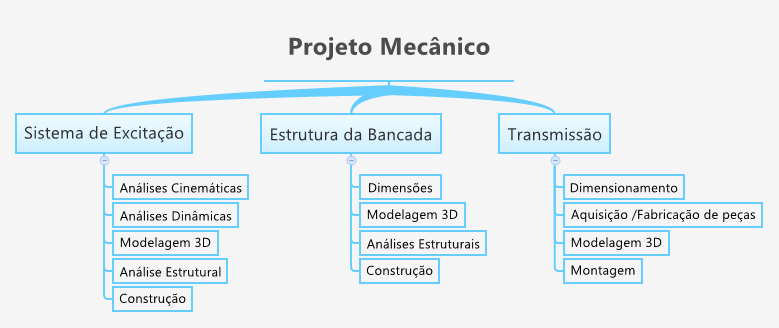
\includegraphics[scale=0.6]{eap-mecanica.png}
		\caption{Estrutura Analítica do Projeto Mecânico}
		\label{eap-energia}
	\end{figure}

	\textbf{Lista É / Não É}

		O produto final é a bancada de teste de amortecedores veiculares. Este produto não são veículos que não sejam leves, que segundo o Código de Trânsito Brasileiro - CTB são veículos com até 3500kg, porém o projeto será mais restrito ainda, trabalhando apenas com amortecedores de veículos leves e populares em que o peso bruto máximo do veículo é 1600Kg.

	\textbf{Requisitos}

		Para atingir o objetivo proposto na área da mecânica, faz-se necessário atender alguns requisitos. Esses requisitos se encontram citados a seguir:

		\begin{itemize}
			\item Possibilidade de troca do curso do amortecedor;
			\item Dimensionamento de peças viáveis para fabricação, de acordo com as ferramentas ao alcance;
			\item Possibilidade de alterar a altura do apoio superior, para se adequar ao tamanho do amortecedor.

		\end{itemize}


	\textbf{Propósito}

		Para realização dos testes em amortecedores, é necessário um sistema de excitação que seja capaz de comprimir e estender o amortecedor de forma que a velocidade possa ser trocada e uma estrutura que resiste as forças do sistema. Com isso é necessário que seja dimensionado tanto o sistema de excitação com diferentes velocidades, quanto uma estrutura que suporte as forças existentes no sistema. 


	\textbf{Cronograma}

		\newpage
		\begin{table}[]
			\centering
			\caption{My caption}
			\label{my-label}
			\resizebox{\textwidth}{!}{%
			\begin{tabular}{ccccc}
			\hline
			\rowcolor[HTML]{FFFFFF} 
			\textbf{ATIVIDADES}                                                                                   & \textbf{RESPONSÁVEL}                                               & \textbf{Data Inicio} & \textbf{Data Fim} & \textbf{\begin{tabular}[c]{@{}c@{}}(\%)\\   Conclusão\end{tabular}} \\ \hline
			Revisão Bibliográfica                                                                                 & \begin{tabular}[c]{@{}c@{}}Breno e Paulo \\ e Larissa\end{tabular} & 25/03                & 27/03             & 100\%                                                               \\ \hline
			Definição de escopo                                                                                   & \begin{tabular}[c]{@{}c@{}}Breno e Paulo \\ e Larissa\end{tabular} & 04/04                & 08/04             & 100\%                                                               \\ \hline
			Propostas de sistema de Excitação                                                                     & \begin{tabular}[c]{@{}c@{}}Breno e Paulo \\ e Larissa\end{tabular} & 11/04                & 15/04             & 100\%                                                               \\ \hline
			Apresentação PC1                                                                                      & Larissa                                                            & 22/04                & 22/04             & 100\%                                                               \\ \hline
			\begin{tabular}[c]{@{}c@{}}Equacionamento da Biela Manviela \\ Analítico\end{tabular}                 & Breno                                                              & 25/04                & 29/04             & 100\%                                                               \\ \hline
			Análises cinemáticas e dinâmicas                                                                      & Larissa                                                            & 02/05                & 06/05             & 100\%                                                               \\ \hline
			Desenhar sistema de excitação                                                                         & Larissa                                                            & 02/05                & 06/05             & 90\%                                                                \\ \hline
			Transmissão                                                                                           & Paulo                                                              & 09/05                & 13/05             & 90\%                                                                \\ \hline
			Análises estruturais                                                                                  & Larissa                                                            & 09/05                & 13/05             & 100\%                                                               \\ \hline
			Revisão do texto do Relatório                                                                         & Larissa                                                            & 16/05                & 25/05             & 100\%                                                               \\ \hline
			Apresentação PC 2                                                                                     & Paulo                                                              & 26/05                & 01/06             & 100\%                                                               \\ \hline
			Contruir parte deslizante da bancada                                                                  & Breno                                                              & 25/05                & 29/05             & 15\%                                                                \\ \hline
			Fabricar Biela e polia da manivela                                                                    & Larissa                                                            & 29/05                & 05/06             & 15\%                                                                \\ \hline
			Adquirir peças da Transmissão                                                                         & Paulo                                                              & 29/05                & 05/06             & 20\%                                                                \\ \hline
			Montar a estrutra                                                                                     & Larissa                                                            & 05/06                & 1206              & 0\%                                                                 \\ \hline
			Montar o sistema de exitação                                                                          & Breno                                                              & 05/06                & 12/06             & 0\%                                                                 \\ \hline
			Montar o sistema de transmissão                                                                       & Paulo                                                              & 05/06                & 12/06             & 0\%                                                                 \\ \hline
			\begin{tabular}[c]{@{}c@{}}Testar o sistema de exitação em\\  conjunto com a trasminssão\end{tabular} & Breno                                                              & 12/06                & 20/06             & 0\%                                                                 \\ \hline
			\end{tabular}%
		}
		\end{table}


	\textbf{Restrições e Riscos}

		Algumas das restrições do projeto mecânico são listadas a seguir:

		\begin{itemize}
			\item Utilização de amortecedores de veículos leves e populares;
			\item Teste em três cursores com diâmetros de 10cm, 12,5cm e 15cm;
			\item Testes nas velocidades: 175mm/s, 200mm/s e 225mm/s;
			\item Torque máximo no motor de 2,91N.m para o cursor de 15cm;
			\item Torque máximo no motor de 2,43N.m para o cursor de 12,5cm;
			\item Torque máximo no motor de 1,94N.m para o cursor de 10cm.
		\end{itemize}

		E alguns riscos são:

		\begin{itemize}
			\item O torque geral do sistema não pode ultrapassar 6,1N.m devido a ser o torque nominal que o motor suporta;
			\item O sistema biela manivela tem que ser de aço 1020, por ser um material mais rígido, isto se deve ao fato de ser a parte da bancada que vai estar mais sujeita a desgaste;
			\item As barras deslizantes tem que ser uma superfície com o mínimo possível de atrito. 
		\end{itemize}



\subsection{Sistema de Transmissão}

	Nesta seção serão mostradas as decisões a respeito do sistema de transmissão, assim como o equacionamento e cálculos referentes a ele.

	\subsubsection{Definições}

		Nessa bancada, temos um motor que deve transmitir seu movimento de rotação para a manivela. Há ainda, a necessidade de multiplicar o torque desse motor, para que ele seja suficiente para movimentar a manivela e o amortecedor. Além disso, é preciso que a velocidade do motor seja reduzida, para que a manivela trabalhe na rotação desejada, com o motor trabalhando em rotações altas, onde tem maior torque.

		Há várias formas de realizar isso, seja por engrenagens, eixos rígidos com caixas de redução, ou correias. Nesse caso, não necessitamos de um sincronismo perfeito entre motor e manivela, sendo assim, o alto custo de um sistema com eixo rígido ou outro com transmissão toda feita por engrenagens, não seria justificado. Pelo mesmo motivo, também não seria justificado o uso de correias dentadas. Por isso, a melhor escolha é uma transmissão por correia do tipo V, com polias de diferentes tamanhos no motor e na manivela. 

		Para o projeto de toda essa transmissão, primeiramente determinou-se as três velocidades lineares e também os três diferentes cursos nos quais o teste seria executado. A decisão desses parâmetros levou em conta vários artigos, e também informações técnicas de amortecedores e de outras máquinas. A tabela \ref{desMecanica001} apresenta as velocidades lineares e os cursos que o amortecedor poderá ser testado.

		\newpage
		\begin{table}[!h]
			\centering
			\caption{Velocidades e cursos de testes do amortecedor}
			\label{desMecanica001}
			\begin{tabular}{|c|c|}
			\hline
			\rowcolor[HTML]{C0C0C0} 
			{\color[HTML]{000000} \textbf{\begin{tabular}[c]{@{}c@{}}Velocidades no\\ Amortecedor(mm/s)\end{tabular}}} & {\color[HTML]{000000} \textbf{Curso(mm)}} \\ \hline
			{\color[HTML]{000000} 225} & {\color[HTML]{000000} 150} \\ \hline
			{\color[HTML]{000000} 200} & {\color[HTML]{000000} 125} \\ \hline
			{\color[HTML]{000000} 175} & {\color[HTML]{000000} 100} \\ \hline
			\end{tabular}
		\end{table}

		São necessárias três velocidades pois, em cada velocidade a força de reação do amortecedor é diferente, e deseja-se plotar um gráfico com esses parâmetros.  Os três cursos diferentes são necessários para simular situações distintas, onde o amortecedor é comprimido ou tracionado com amplitudes diferentes. A variação do curso também é essencial no âmbito didático da bancada, pois com isso pode-se mostrar na prática que o curso de amortecimento não influencia na força exercida pelo amortecedor, e que somente a variação das velocidades causa uma variação na força de reação.

		Com os cursos e velocidades definidos, analiticamente, percebeu-se que para garantir que o motor trabalhasse em altas rotações para que tivesse um bom torque, seria necessário o uso de uma caixa de redução, pois para fazer essa redução somente nas polias, a polia do motor teria que ser muito pequena e a da manivela muito grande. 

		A diferença muito grande de diâmetros das polias não é desejável pois polias muito pequenas tem menor agarramento na correia, e uma polia muito grande na manivela tornaria a máquina enorme, elevando o custo de forma significativa.

		Esses aspectos foram levados em conta também na hora de escolher a capacidade de redução do componente. Foi então determinado o uso de uma caixa de redução de 1:12 assim como ilustra a figura \ref{desMecanica002}, com eixos de entrada e saída paralelos, onde serão instaladas polias de mesmo tamanho.

		\begin{figure}[h]
			\centering
			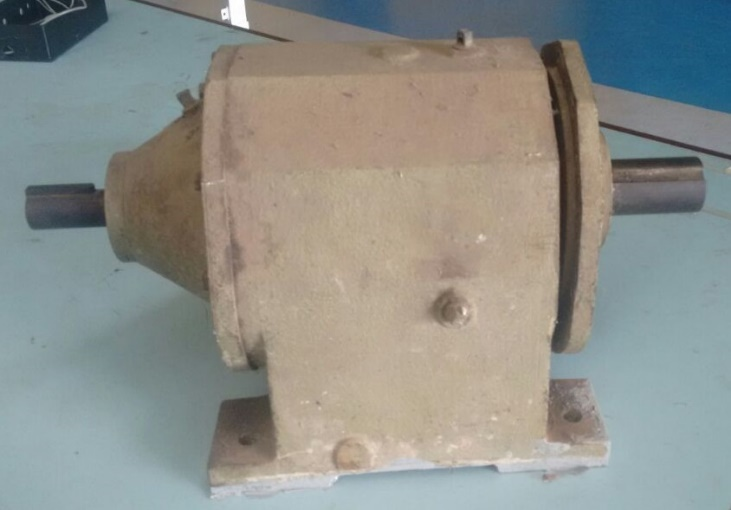
\includegraphics[scale=1]{desMecanica002}
			\caption{Caixa de redução de 1:12}
			\label{desMecanica002}
		\end{figure}

		Com os valores de redução, consegue-se realizar o restante da redução dimensionando adequadamente o valor das polias da manivela e do motor, sem que as mesmas sejam de tamanhos inadequados ao projeto.

		De forma geral e com intuito de facilitar a visualização do sistema de transmissão, foi feito um esboço do mesmo, mostrado na figura \ref{desMecanica003}.

		\begin{figure}[h]
			\centering
			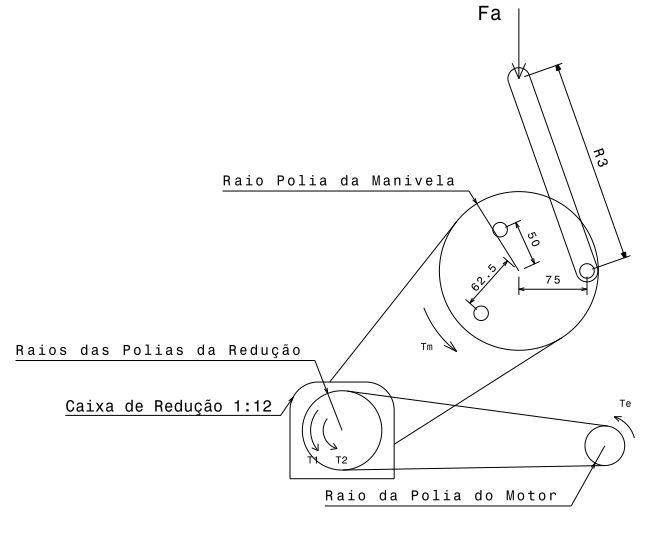
\includegraphics[scale=0.9]{desMecanica003}
			\caption{Esboço do sistema de transmissão}
			\label{desMecanica003}
		\end{figure}

		Onde:
		\begin{itemize}
			\item $R_{3}$:Comprimento da biela
			\item $F_{a}$:Força de reação exercida pelo amortecedor
			\item $T_{m}$: Torque na manivela
			\item $T_{1}$: Torque na entrada da caixa de redução
			\item $T_{2}$: Torque na saída da caixa de redução
			\item $T_{e}$: Torque no motor
		\end{itemize}

		O equacionamento do sistema de transmissão inicia-se com a relação entre os torques e as velocidades na entrada e na saída da caixa de redução, onde V1 e V2 correspondem com a velocidade de rotação de entrada e saída da caixa de redução, respectivamente. As equações (5.1) e (5.2) mostram as relações de 1:12 para torque e velocidade.

		\begin{equation}
			 T_{2}=12 \times T_{1} 
		\end{equation}
		
		\begin{equation}
			 V_{1}=12 \times V_{2} 
		\end{equation}

		Assumiu-se também que as duas polias da caixa de redução serão do mesmo tamanho. Assim, tornou-se necessário o valor da velocidade linear que será utilizada, para isso calculou-se inicialmente a velocidade linear na situação em que haverá a maior velocidade angular da manivela, que é o teste com curso de 100 mm e velocidade 225mm/s no amortecedor. 

		Sendo assim, para esse caso deveremos ter a maior velocidade de rotação desejada no motor, que é de 1350rpm. Através de um programa no MATLAB, que será melhor explicado na seção ANÁLISES DINAMICAS, foi obtida a velocidade angular de 41,95 rpm da manivela, que nesse curso, nos proporcionaria a velocidade de 225mm/s no amortecedor. Assim foi possível calcular a relação das polias de acordo coma a equação 3.

		\begin{equation}
			\frac{41,9 \times 12}{1350}= \frac{ d_{e}}{d_m}
		\end{equation}

		Portanto, a relação de diâmetros deve ser de:

		\begin{equation}
			2.68=\frac{ d_{e}}{d_m}
		\end{equation}

		Para o cálculo do torque no motor, é necessário saber primeiramente qual a força de reação máxima que o amortecedor aplicará. Sabe-se que será na velocidade de 225mm/s, e com o curso de 15cm. Com base em alguns artigos e trabalhos na área, focando em gráficos de força x velocidade, assumiu-se que a força média que um amortecedor aplica respondendo a essa velocidade é de 1250N. É importante salientar que esse valor varia de acordo com o tipo de amortecedor, temperatura em que o mesmo se encontra, estado de utilização, entre outros fatores. Tem-se então o torque máximo na manivela:

	
		$$T_{m}= {1250 \times 0,075} = 93,75 {\frac{N}{m}}$$
	

		Usando (5.1) e (5.4) e fazendo a relação entre torques devido a relação de diâmetro entre as polias da manivela e do motor obtém-se a equação 5

		\begin{equation}
			T_{e}= {\frac{T_{m}}{32,12}}
		\end{equation}

		Assim chega-se ao torque máximo que o sistema irá gerar no motor, de 2,918 N.m.

		Utilizando esse mesmo procedimento mostrado, foi montada a figura \ref{desMecanica004} com os valores para cada velocidade e cada curso.

		\begin{figure}[h]
			\centering
			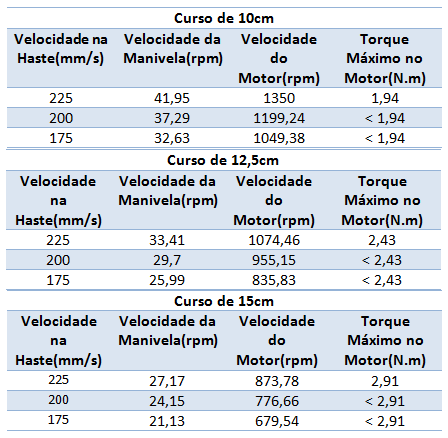
\includegraphics[scale=1]{desMecanica004}
			\caption{Valores de velocidade para cada curso}
			\label{desMecanica004}
		\end{figure}

\subsection{Análises}
	
	Nesta seção serão mostradas as análises realizadas no projeto, que foram divididas em análise dinâmica, realizada em ambiente multicorpos no software  Adams/Car, e análises estáticas, realizadas no software ANSYS para o dimensionamento de peças. 

	\subsubsection{Equacionamento Biela-Manivela}

		Com o propósito de analisar o sistema biela manivela, utilizou-se o método de números complexos para determinar as equações cinemáticas e dinâmicas do sistema, com isto foi possível determinar alguns parâmetros importantes, como velocidade e aceleração por exemplo. Utilizou-se o MatLab®, para representar graficamente os resultados.

		O deslocamento do pistão descreve um movimento oscilatório, que é considerado um movimento harmônico simples, onde plotado o deslocamento pelo tempo ou pelo ângulo de inclinação da manivela, gera uma função seno.

		De forma geral o sistema biela manivela de uma máquina é mostrado na figura \ref{desMecanica005}, e suas devidas partes são detalhadas a seguir. Vale ressaltar que para os cálculos da posição, utilizou-se a nomenclatura da mesma figura.

		\begin{figure}[!h]
			\centering
			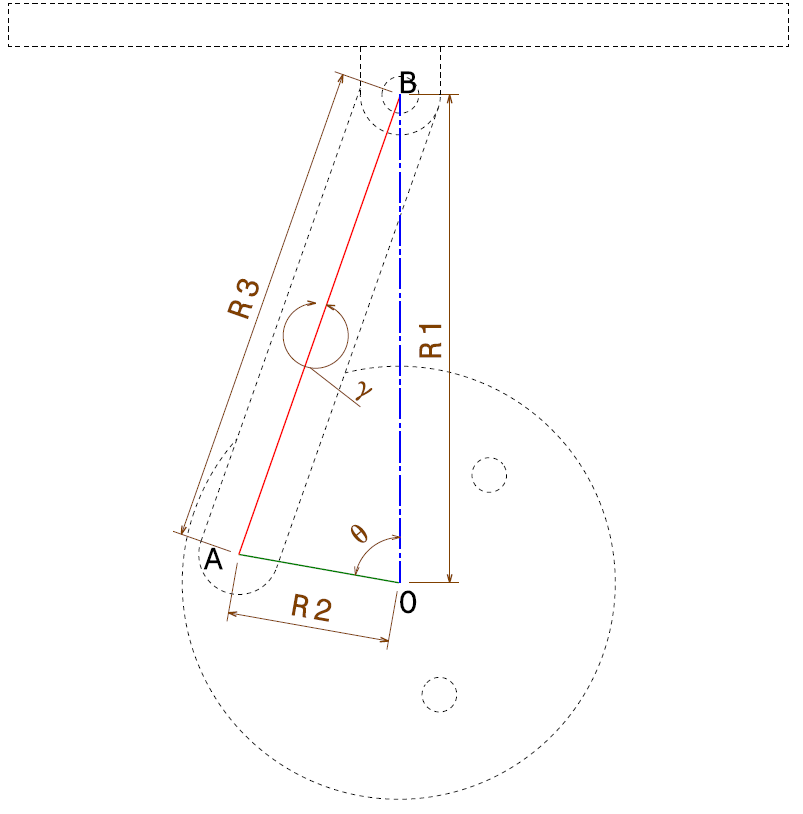
\includegraphics[scale=0.5]{desMecanica005}
			\caption{Esboço do Mecanismo Biela-Manivela}
			\label{desMecanica005}
		\end{figure}

		Onde:
		\begin{itemize}
			\item $ \overline{OA} $ = R2: Manivela (descreve uma circunferência de raio $ \overline{OB} $);
			\item $ \overline{BA} $ = R3: Comprimento da biela; 
			\item $A$: Base de biela (deslocado ao longo de uma reta, ou seja, o cursor);
			\item $B$: Cabeça de biela (articulado em B);
			\item $\theta$: Ângulo da Manivela com a Vertical;
			\item $\gamma$: Ângulo que a Biela pode vir a percorrer
		\end{itemize}

		Através do método dos números complexos em formato polar, figura \ref{desMecanica006}, tem-se a equação cíclica:

		\begin{figure}[h]
			\centering
			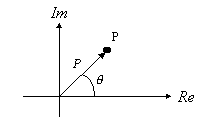
\includegraphics[scale=1]{desMecanica006}
			\caption{Notação de números complexos em formato polar}
			\label{desMecanica006}
		\end{figure}

		Assim:

		\begin{equation}
			R_{1} = R_{2} + R_{3}
		\end{equation}

		As equações acima possuem componentes reais e imaginários, com isto a Equação (5.6) foi separada em duas partes: 

		\textbf{Componente Real:}

		\begin{equation}
			R_{1r} = R_{2}(cos(\theta)) + R_{3}(cos(\gamma))
		\end{equation}

		\textbf{Componente Imaginário:}

		\begin{equation}
			R_{1i} = R_{2}(sen(\theta)) + R_{3}(sen(\gamma))
		\end{equation}

		Ao aplicar a lei dos senos, isola-se $\theta{3}$, obtendo assim a Equação (5.8):

		\begin{equation}
			\gamma = sen^{-1} ( - \frac{R_{2}}{R_{3}}(sen\theta))
		\end{equation}

		Ao derivar a Equações (5.9) obtém as velocidades real e imaginária, assim:

		\textbf{Componente Real:}

		\begin{equation}
			V_{1r} = -R_{2}w_{2}(sen(\theta)) - R_{3}w_{3}(sen(\gamma))
		\end{equation}

		\textbf{Componente Imaginário:}

		\begin{equation}
			V_{1i} = 0 = R_{2}w_{2}(cos(\theta)) - R_{3}w_{3}(cos(\gamma))
		\end{equation}

		Ao isolar a velocidade angular da barra 3, se obtem a seguinte Equação (5.12):

		\begin{equation}
			w_{3} = - w_{2} (\frac{R_{2}cos(\theta)}{R_{3}cos(\gamma)})
		\end{equation}

	\subsubsection{Análise Dinâmica}

		O mecanismo biela manivela é utilizado para transformação de um movimento de rotação em movimento linear, esse sistema tem diversas aplicações na engenharia, como em motores e locomotivas. Na figura \ref{desMecanica007} é apresentado o sistema biela manivela que será utlizado na bancada e as variáveis utilizadas para o equacionamento.

		\begin{figure}[h]
			\centering
			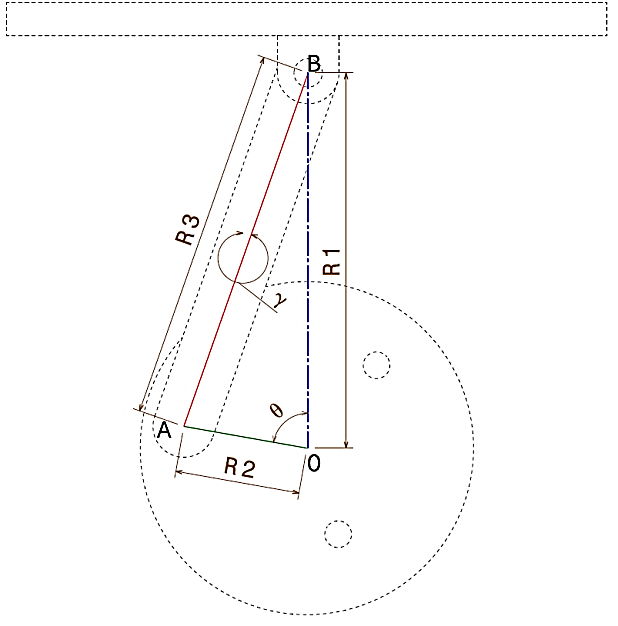
\includegraphics[scale=1.4]{desMecanica007}
			\caption{Esboço Mecanismo Biela-Manivela}
			\label{desMecanica007}
		\end{figure}

		O curso do sistema biela manivela é a diferença entre a distância máxima e mínima que o pistão alcança, no caso da bancada o pistão é o apoio do amortecedor localizado no ponto B da figura \ref{desMecanica007}. Como requisito de projeto a bancada deve ser capaz de ajustar o curso para cada tamanho de amortecedor, portanto o tamanho R2 deve ser variado, o que pode ser feito fixando o ponto A na posição 1, como está fixado na figura \ref{desMecanica007}, posição 2 ou 3.

		A alteração do diâmetro da manivela altera também a velocidade linear no ponto B, portanto para cada curso faz-se necessário uma velocidade de rotação diferente para manter as mesmas velocidades lineares em diferentes cursos.  

		Com o propósito de analisar o sistema biela manivela no seu comportamento cinemático utilizou-se o equacionamento do sistema, com isto foi possível determinar a velocidade de rotação e o comprimento dos seus componentes, que influenciam na velocidade linear da placa que o amortecedor se encontra fixo. Utilizou-se o MatLab®, para representar graficamente os resultados e para validação da velocidade encontrada analiticamente foi utilizado o software Adams/Car.

		Na figura \ref{desMecanica008} é apresentada o gráfico de deslocamento linear em função do ângulo da manivela, como entrada do programa foi informado o comprimento da biela, comprimento da manivela e velocidade angular na manivela.

		\begin{figure}[h]
			\centering
			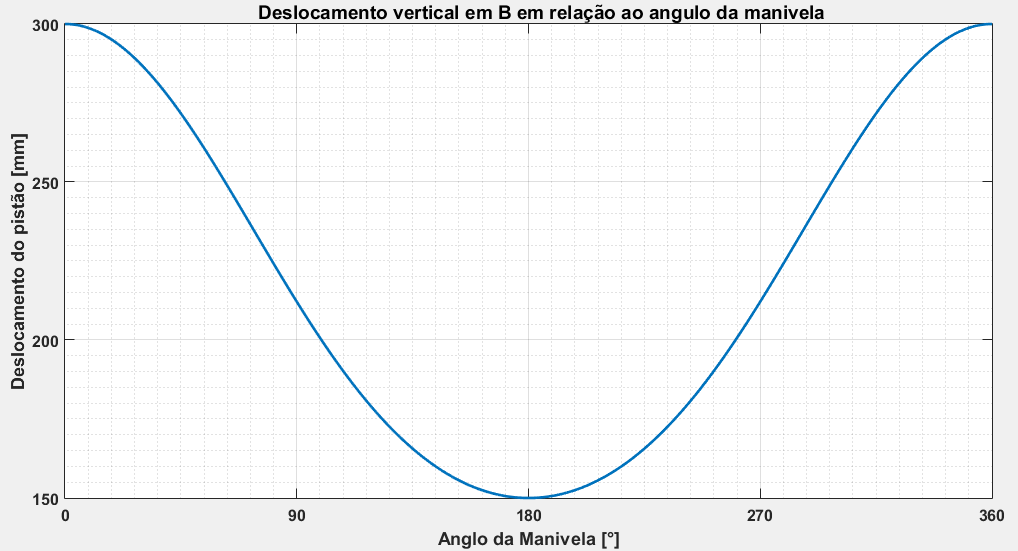
\includegraphics[scale=0.4]{desMecanica008}
			\caption{Deslocamento do ponto B x Ângulo da manivela}
			\label{desMecanica008}
		\end{figure}

		Com os mesmos dados de entrada foi plotado o valor da velocidade linear do ponto B em relação ao ângulo da manivela, apresentado da figura \ref{desMecanica009}.

		\begin{figure}[h]
			\centering
			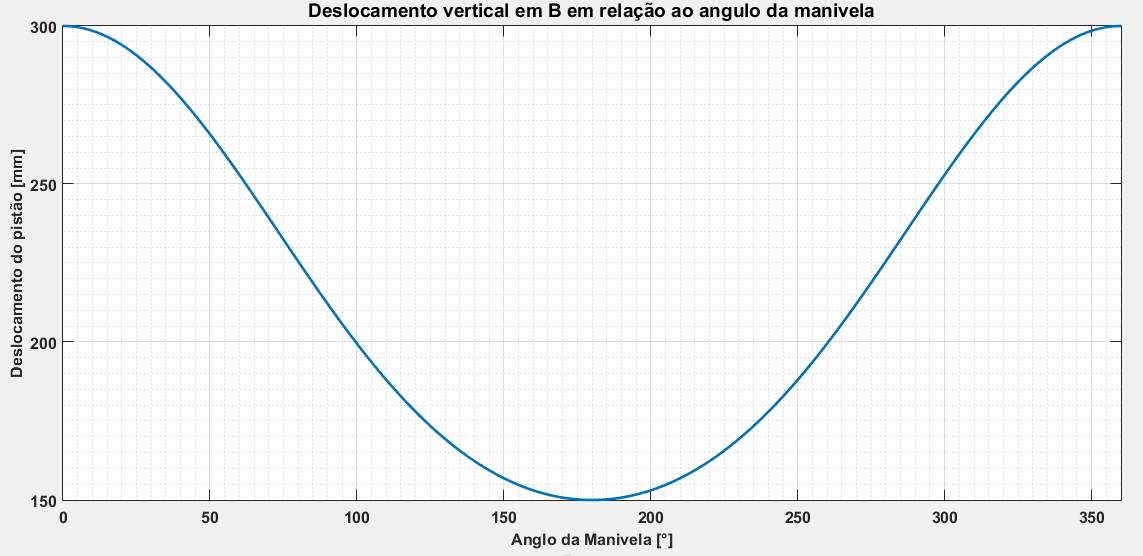
\includegraphics[scale=0.4]{desMecanica009}
			\caption{Velocidade linear no ponto B x ângulo da manivela}
			\label{desMecanica009}
		\end{figure}

		Com os dados de entradas mostrados na figura \ref{desMecanica010} a velocidade máxima linear atingida em B foi de 230 mm/s.

		\begin{figure}[h]
			\centering
			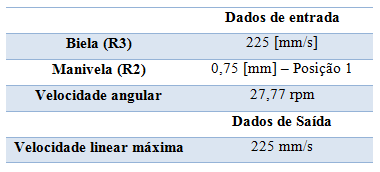
\includegraphics[scale=1]{desMecanica010}
			\caption{Dados de entrada no programa}
			\label{desMecanica010}
		\end{figure}

		A validação realizada no software Adams/Car, utiliza elementos rígidos para uma análise multicorpos que é uma técnica que resolve equações de cinemática, estática, e dinâmica de sistemas com vários corpos e muitos graus de liberdade. Cada elemento criado na modelagem inicia com seis graus de liberdade, e cada junta restringe os graus de liberdade. Foram utilizadas três juntas de rotação, uma junta de translação e uma junta fixa.

		O sistema modelado é apresentado na figura \ref{desMecanica011}, apresentando os quatro elementos utilizados para a modelagem, três juntas de rotação, uma junta fixa e uma junta translacional. Também foi adicionado um movimento rotacional no elemento em vermelho com velocidade angular de 27,77 rpm e a velocidade linear foi medida no bloco azul, que no esquema da figura \ref{desMecanica011} representa o ponto B. Para retirar as forças exercidas em cada junta o peso do bloco azul foi alterado para o peso estimado do sistema.

		\begin{figure}[!h]
			\centering
			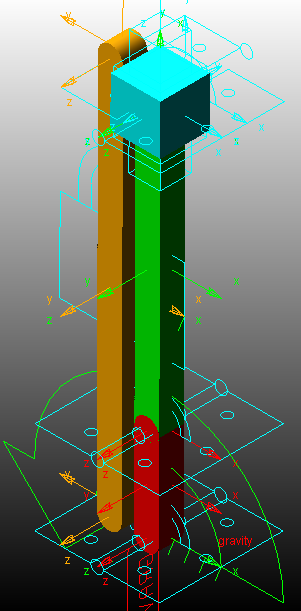
\includegraphics[scale=0.35]{desMecanica011}
			\caption{Modelagem multicorpos}
			\label{desMecanica011}
		\end{figure}

		De acordo com as velocidades escolhidas na seção de transmissão, foram validadas as velocidades de rotação para cada velocidade escolhida e cada curso. Como serão três cursos e cada um desses deve operar em três velocidades, serão nove rotações diferentes na manivela. 
		
		Os gráficos de deslocamento e velocidade no software Adams/Car tiveram resultados iguais aos do MatLab, como a velocidade é a variável que motivou a análise, a figura \ref{desMecanica012} apresenta o gráfico do software Adams/car de velocidade linear no ponto B em função do ângulo da manivela, onde a velocidade linear máxima foi de 225 mm/s.

		\begin{figure}[!h]
			\centering
			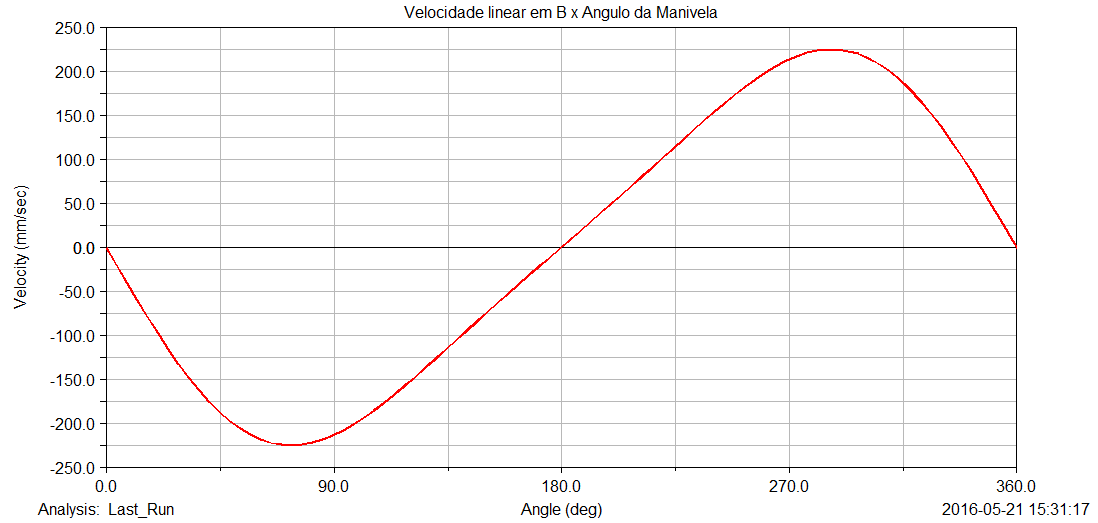
\includegraphics[scale=0.35]{desMecanica012}
			\caption{Velocidade linear em B x Ângulo da manivela}
			\label{desMecanica012}
		\end{figure}

		No mesmo modelo do Adams/Car foi possível retirar as forças máximas em x e y considerando um bloco com peso de 200 kg. As forças encontradas foram retiradas por eixo, onde as máximas em x se encontram quando o ângulo de 90 e 270 graus com a vertical, como mostra o gráfico da figura \ref{desMecanica013}.

		
		\begin{figure}[!h]
			\centering
			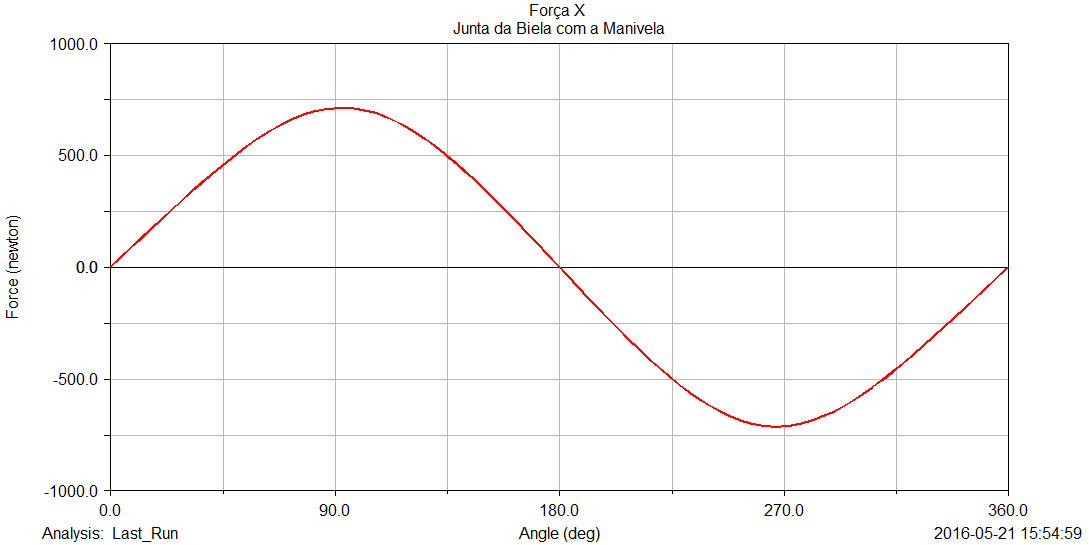
\includegraphics[scale=0.35]{desMecanica013}
			\caption{Força máxima no eixo X no ponto A}
			\label{desMecanica013}
		\end{figure}

		Já a força máxima no ponto A no eixo Y ocorre quando o ângulo da manivela é 0 e 360, como mostra o gráfico na figura \ref{desMecanica014}.

		\begin{figure}[!h]
			\centering
			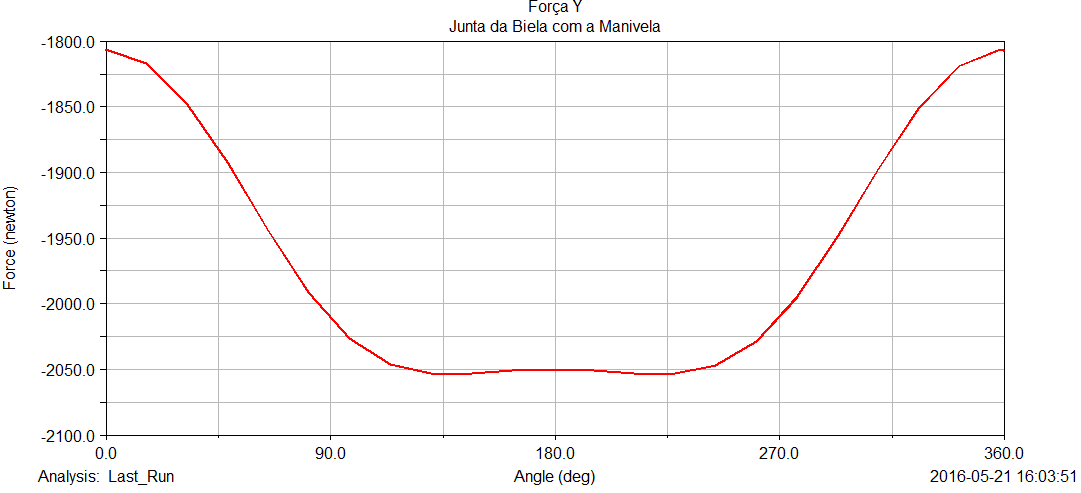
\includegraphics[scale=0.35]{desMecanica014}
			\caption{Força máxima no eixo Y no ponto A}
			\label{desMecanica014}
		\end{figure}

		Com as forças dinâmicas do sistema modelado no software Adams/Car é possível fazer a análise estrutural das peças que estão sofrendo pela ação dessas forças. A figura \ref{desMecanica015} mostra os valores encontrados de força máxima.

		\begin{figure}[!h]
			\centering
			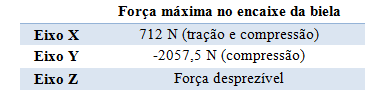
\includegraphics[scale=1]{desMecanica015}
			\caption{Forças Dinâmicas}
			\label{desMecanica015}
		\end{figure}

	\subsubsection{Análises Estruturais}

		Para a análise estrutural das peças faz-se necessário a escolha dos materiais da bancada, geometria das peças, e forças dinâmicas atuantes na mesma. Na seção anterior foi descrita a metodologia para obtenção das forças dinâmicas, a geometria foi modelada no software CATIA V5 e os materiais estão apresentados na figura \ref{desMecanica016}.

		\begin{figure}[!h]
			\centering
			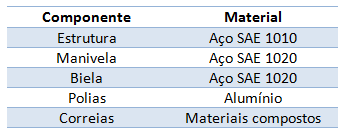
\includegraphics[scale=1]{desMecanica016}
			\caption{Material dos Componentes escolhidos para a bancada}
			\label{desMecanica016}
		\end{figure}

		Para a fase em andamento do projeto, foi analisada somente a biela, peça que está submetida a transmissão de forças da manivela para o amortecedor. A estrutura ainda deve ser analisada em uma simulação de vibração e estrutural.
		
		Com o resultado das análises dinâmicas realizadas, será verificada as tensões nas peças que estão sofrendo as forças retiradas na seção anterior, considerando a biela feita com Aço SAE 1020, que possui tensão de escoamento 210 MPa.
		
		Como o teste é cíclico, além de avaliar as tensões equivalentes de von-Mises e deslocamento máximo, também será analisada a vida da peça em fadiga e seu coeficiente de segurança. 
		
		A parte crítica da bancada é a biela, onde transmite a força da manivela para o amortecedor, portanto será simulada pelo método de elementos finitos. 
		
		As análises feitas para as três velocidades, de 225 mm/s, 200 mm/s e 175 mm/s, e os três cursos, de 150 mm, 125mm e 100 mm, foram realizadas e os resultados que serão utilizados para as análises serão os valores críticos no eixo X e no eixo Y. A figura \ref{desMecanica017} apresenta os valores encontrados nas análises dinâmicas.

		\begin{figure}[!h]
			\centering
			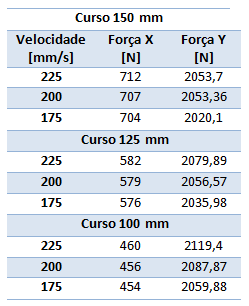
\includegraphics[scale=1]{desMecanica017}
			\caption{Forças dinâmicas do Sistema Biela-Manivela}
			\label{desMecanica017}
		\end{figure}

		A força máxima encontrada no eixo X foi no maior curso, 150mm, e maior velocidade, 225 mm/s. Essas forças serão utilizadas para a análise da biela. A figura \ref{desMecanica018} apresenta o CAD da biela.

		\newpage
		\begin{figure}[!h]
			\centering
			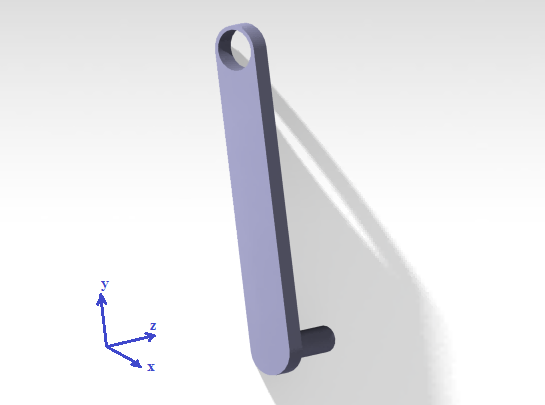
\includegraphics[scale=0.8]{desMecanica018}
			\caption{CAD da Biela}
			\label{desMecanica018}
		\end{figure}

		A simulação da força no eixo X foi realizada com a parte superior engastada e a força aplicada no pino de encaixe com a manivela. Como as forças foram retiradas em uma análise dinâmica, não será adicionado um fator dinâmico às forças encontradas.
		
		A figura \ref{desMecanica019} apresenta a tensão equivalente de von-Mises para a biela com a força aplicada de 712 N no eixo X. A tensão máxima atingiu 45,957 Mpa, não atingindo o escoamento.

		\newpage
		\begin{figure}[!h]
			\centering
			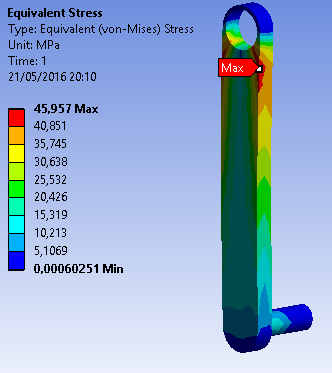
\includegraphics[scale=0.8]{desMecanica019}
			\caption{Tensão equivalente de von-Mises para Fx}
			\label{desMecanica019}
		\end{figure}

		Mas como a força X é alternada e cíclica, é necessário verificar a fadiga, onde a barra atingiu a vida de 106 ciclos, que é considerada vida infinita, e o menor coeficiente de segurança de 1,87, como mostra a figura \ref{desMecanica020}. 

		\newpage
		\begin{figure}[!h]
			\centering
			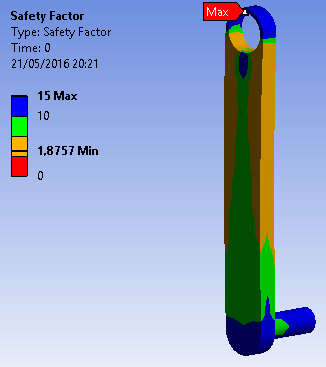
\includegraphics[scale=0.8]{desMecanica020}
			\caption{Coeficiente de segurança para fadiga}
			\label{desMecanica020}
		\end{figure}

		Para a força y, como não é alternada, é somente em um sentido, foi realizada com a máxima força encontrada, na situação com o menor curso e maior velocidade, que a força atinge 2119,4 N. A figura \ref{desMecanica021} apresenta o resultado da tensão equivalente de von-Mises.

		\newpage
		\begin{figure}[!h]
			\centering
			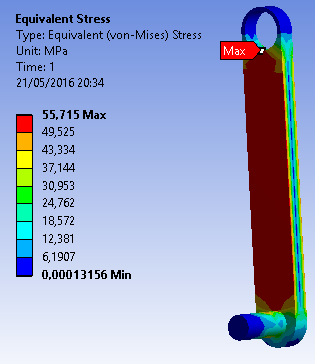
\includegraphics[scale=0.8]{desMecanica021}
			\caption{Tensão equivalente de von-Mises para Fy}
			\label{desMecanica021}
		\end{figure}

		A análise com a força Y atingiu 55,71 MPa, onde não atinge o escoamento do aço 1020.










